% Options for packages loaded elsewhere
\PassOptionsToPackage{unicode}{hyperref}
\PassOptionsToPackage{hyphens}{url}
\PassOptionsToPackage{dvipsnames,svgnames,x11names}{xcolor}
\documentclass[
  a4paper,
  zihao=5,
  fontset=none]{ctexart}
\usepackage{xcolor}
\usepackage[top=2.45cm,bottom=2.2cm,left=1.95cm,right=1.95cm,headheight=16pt,includehead]{geometry}
\usepackage{amsmath,amssymb}
\setcounter{secnumdepth}{-\maxdimen} % remove section numbering
\usepackage{iftex}
\ifPDFTeX
  \usepackage[T1]{fontenc}
  \usepackage[utf8]{inputenc}
  \usepackage{textcomp} % provide euro and other symbols
\else % if luatex or xetex
  \usepackage{unicode-math} % this also loads fontspec
  \defaultfontfeatures{Scale=MatchLowercase}
  \defaultfontfeatures[\rmfamily]{Ligatures=TeX,Scale=1}
\fi
\usepackage{lmodern}
\ifPDFTeX\else
  % xetex/luatex font selection
\fi
% Use upquote if available, for straight quotes in verbatim environments
\IfFileExists{upquote.sty}{\usepackage{upquote}}{}
\IfFileExists{microtype.sty}{% use microtype if available
  \usepackage[]{microtype}
  \UseMicrotypeSet[protrusion]{basicmath} % disable protrusion for tt fonts
}{}
\makeatletter
\@ifundefined{KOMAClassName}{% if non-KOMA class
  \IfFileExists{parskip.sty}{%
    \usepackage{parskip}
  }{% else
    \setlength{\parindent}{0pt}
    \setlength{\parskip}{6pt plus 2pt minus 1pt}}
}{% if KOMA class
  \KOMAoptions{parskip=half}}
\makeatother
\usepackage{longtable,booktabs,array}
\newcounter{none} % for unnumbered tables
\usepackage{calc} % for calculating minipage widths
% Correct order of tables after \paragraph or \subparagraph
\usepackage{etoolbox}
\makeatletter
\patchcmd\longtable{\par}{\if@noskipsec\mbox{}\fi\par}{}{}
\makeatother
% Allow footnotes in longtable head/foot
\IfFileExists{footnotehyper.sty}{\usepackage{footnotehyper}}{\usepackage{footnote}}
\makesavenoteenv{longtable}
\setlength{\emergencystretch}{3em} % prevent overfull lines
\providecommand{\tightlist}{%
  \setlength{\itemsep}{0pt}\setlength{\parskip}{0pt}}
\definecolor{ink}{HTML}{1F2329}
\definecolor{gold}{HTML}{C9A227}
\definecolor{golddeep}{HTML}{A97820}
\definecolor{cream}{HTML}{FBF6EE}
\definecolor{paper}{HTML}{F7F1E6}
\definecolor{line}{HTML}{E7D3AE}
\definecolor{terra}{HTML}{C45C26}
\definecolor{muted}{HTML}{86909C}
\definecolor{rule}{HTML}{F0E2C8}

\setmainfont{TeX Gyre Pagella}
\setmonofont{Consolas}[Scale=0.88]
\setCJKmainfont{DengXian}[AutoFakeBold=2.4, AutoFakeSlant=0.15]
\setCJKsansfont{Microsoft YaHei}[AutoFakeBold=2.2]
\setCJKmonofont{DengXian}[Scale=0.92]
\newCJKfontfamily\zhsong{STZhongsong}[AutoFakeBold=1.5]
\newfontfamily\coverlatin{TeX Gyre Pagella}

\usepackage{graphicx}
\graphicspath{{d:/ai-banking-agent/BankingMiniprogram/images/}}
\usepackage{tikz}
\usetikzlibrary{arrows.meta,positioning}
\usepackage{caption}
\captionsetup{font=small,labelfont={bf,color=golddeep},textfont={color=ink},skip=8pt,labelsep=quad}
\usepackage{fancyhdr}
\usepackage{enumitem}
\setlist[enumerate]{itemsep=0.28em,topsep=0.4em,leftmargin=1.6em}
\setlist[itemize]{itemsep=0.28em,topsep=0.4em,leftmargin=1.4em}

\usepackage{titlesec}
\newcommand{\zhsectionrule}{\vspace{-1pt}\begingroup\color{gold}\titlerule[0.7pt]\endgroup}
\titleformat{\section}{\zihao{3}\zhsong\color{ink}}{}{0pt}{}[\zhsectionrule]
\titleformat{\subsection}{\zihao{4}\bfseries\color{golddeep}}{}{0pt}{}
\titleformat{\subsubsection}{\zihao{-4}\bfseries\color{ink}}{}{0pt}{}
\titlespacing*{\section}{0pt}{1.15em}{0.7em}
\titlespacing*{\subsection}{0pt}{0.95em}{0.45em}
\titlespacing*{\subsubsection}{0pt}{0.8em}{0.35em}

\setcounter{tocdepth}{3}
\renewcommand{\contentsname}{目\quad 录}

\renewcommand{\topfraction}{0.92}
\renewcommand{\bottomfraction}{0.4}
\renewcommand{\textfraction}{0.07}
\renewcommand{\floatpagefraction}{0.7}
\linespread{1.18}\selectfont
\emergencystretch=2.5em
\tolerance=1800

\usepackage{etoolbox}
\AtBeginEnvironment{longtable}{\small\renewcommand{\arraystretch}{1.28}}
\AtBeginEnvironment{tabular}{\small\renewcommand{\arraystretch}{1.28}}
\usepackage{colortbl}
\arrayrulecolor{line}

\pagestyle{fancy}
\fancyhf{}
\fancyhead[L]{\footnotesize\color{golddeep}智汇银行}
\fancyhead[R]{\footnotesize\color{muted}智能服务系统技术说明书}
\fancyfoot[C]{\footnotesize\color{golddeep}\thepage}
\renewcommand{\headrulewidth}{0.4pt}
\renewcommand{\headrule}{\hbox to\headwidth{\color{line}\leaders\hrule height \headrulewidth\hfill}}
\renewcommand{\footrulewidth}{0pt}
\fancypagestyle{plain}{%
  \fancyhf{}%
  \fancyhead[L]{\footnotesize\color{golddeep}智汇银行}%
  \fancyhead[R]{\footnotesize\color{muted}智能服务系统技术说明书}%
  \fancyfoot[C]{\footnotesize\color{golddeep}\thepage}%
  \renewcommand{\headrulewidth}{0.4pt}%
  \renewcommand{\headrule}{\hbox to\headwidth{\color{line}\leaders\hrule height \headrulewidth\hfill}}%
}
\usepackage{bookmark}
\IfFileExists{xurl.sty}{\usepackage{xurl}}{} % add URL line breaks if available
\urlstyle{same}
\hypersetup{
  colorlinks=true,
  linkcolor={golddeep},
  filecolor={Maroon},
  citecolor={Blue},
  urlcolor={terra},
  pdfcreator={LaTeX via pandoc}}

\author{}
\date{}

\begin{document}

\definecolor{coverpaper}{HTML}{FBF8F2}
\definecolor{coverink}{HTML}{2C261F}
\definecolor{covergold}{HTML}{8C6A3D}
\definecolor{coverline}{HTML}{D9C4A0}
\definecolor{covermuted}{HTML}{8A8178}

\begin{titlepage}
\thispagestyle{empty}
\pagecolor{coverpaper}
\begin{tikzpicture}[remember picture,overlay]
  \fill[coverpaper] (current page.south west) rectangle (current page.north east);
  \fill[covergold] (current page.north west) rectangle ([yshift=-1.15pt]current page.north east);
  \draw[coverline, line width=0.35pt] ([xshift=18mm,yshift=-16mm]current page.north west) -- ([xshift=-18mm,yshift=-16mm]current page.north east);
  \draw[coverline, line width=0.35pt] ([xshift=18mm,yshift=14mm]current page.south west) -- ([xshift=-18mm,yshift=14mm]current page.south east);
\end{tikzpicture}
\vspace*{22mm}
\begin{center}
\includegraphics[width=1.85cm]{logo-mark.png}\\[10mm]
{\coverlatin\fontsize{11}{14}\selectfont\addfontfeatures{LetterSpace=28}\color{covergold}ZHIHUI BANK}\\[7mm]
{\zhsong\fontsize{42}{50}\selectfont\addfontfeatures{LetterSpace=16}\color{coverink}智汇银行}\\[5.5mm]
{\color{covergold}\rule{2.4cm}{0.6pt}}\\[7mm]
{\zhsong\fontsize{20}{28}\selectfont\color{coverink}智能服务系统技术说明书}\\[3.6mm]
{\zihao{-4}\color{covermuted}内部技术汇报}
\end{center}
\vfill
\begin{center}
{\color{coverline}\rule{9.2cm}{0.4pt}}\\[6mm]
{\coverlatin\fontsize{16}{20}\selectfont\addfontfeatures{LetterSpace=10}\color{covergold}miyomi}\\[3.2mm]
{\zihao{4}\color{coverink}2026年11月1日}\\[2.8mm]
{\zihao{5}\color{covermuted}零售业务\quad\textperiodcentered\quad 金融科技\quad\textperiodcentered\quad 风险管理与信息安全}\\[2mm]
{\small\color{covermuted}依据现行系统实现编制，供内部评审使用}\\[8mm]
{\small\color{covergold}自然语言受理\quad\textperiodcentered\quad 规则引擎裁决\quad\textperiodcentered\quad 客户确认后入账}
\end{center}
\vspace*{18mm}
\end{titlepage}
\nopagecolor
\clearpage
{
\hypersetup{linkcolor=golddeep}
\tableofcontents
}
\clearpage

\subsection{编制说明}\label{ux7f16ux5236ux8bf4ux660e}

本文档说明系统的总体结构、关键算法和安全控制。文中参数、流程和阈值均以现行代码为准。本系统定位为对话式零售银行演示系统，用于验证``自然语言受理、规则引擎裁决、客户确认后入账''的业务闭环。演示环境的控制强度与生产系统不同，文中在安全设计部分分别列明。

\subsection{1.
建设目标与设计原则}\label{ux5efaux8bbeux76eeux6807ux4e0eux8bbeux8ba1ux539fux5219}

系统面向零售客户，在微信小程序中以对话方式办理查询、转账、银行卡管理、代扣管理、风险测评、理财咨询与申购，以及心愿备用金。年长客户可使用大字号界面和语音播报，并可绑定紧急联系人。

设计上坚持四条原则。

\begin{enumerate}
\def\labelenumi{\arabic{enumi}.}
\tightlist
\item
  \textbf{模型负责理解，规则负责裁决。}
  大模型选择工具并组织话术。余额、限额、卡片状态、风险等级、赎回日和是否入账，由服务端程序判定。
\item
  \textbf{展示与办理分离。}
  查询类请求返回业务卡片。转账、申购、资金划转和限额调整先生成待确认指令，客户在确认卡上核对并输入交易密码后，服务端才改写账务。
\item
  \textbf{适当性前置。}
  客户没有一年内有效的风险测评时，系统可以展示理财画像，但不得展示可投货架、出具配置建议或生成申购确认单。
\item
  \textbf{话术不得替代事实。}
  模型未调用工具时，不得向客户声称已经办理、已经冻结或已经生成确认单。语义审核发现此类表述时，改写为尚未执行。
\end{enumerate}

\subsection{2. 系统架构}\label{ux7cfbux7edfux67b6ux6784}

\subsubsection{2.1 逻辑架构}\label{ux903bux8f91ux67b6ux6784}

系统分为四个层次：渠道层、接入层、智能编排层、业务与数据层。模型推理调用外部推理服务，账务与风控留在本系统内。

\begin{figure}[htbp]
\centering
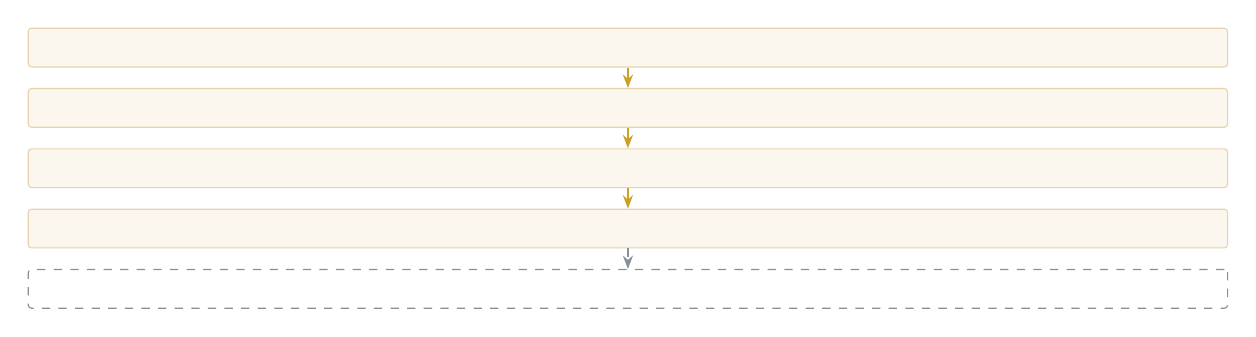
\begin{tikzpicture}[
  font=\small,
  band/.style={draw=line, fill=cream, rounded corners=1.2pt, text width=14.6cm, align=left, inner xsep=9pt, inner ysep=7pt},
  outside/.style={draw=muted, dashed, fill=white, rounded corners=1.2pt, text width=14.6cm, align=left, inner xsep=9pt, inner ysep=7pt},
  node distance=2.6mm
]
  \node[band] (l1) {\textbf{\color{golddeep}渠道层}\enspace 微信小程序：对话、确认卡、适老版字号与语音播放};
  \node[band, below=of l1] (l2) {\textbf{\color{golddeep}接入层}\enspace 登录与会话校验、对话、指令确认与撤销、风险测评、提醒、语音};
  \node[band, below=of l2] (l3) {\textbf{\color{golddeep}智能编排层}\enspace 统一助手、主模型工具调用、语义审核、工具层参数与合规校验};
  \node[band, below=of l3] (l4) {\textbf{\color{golddeep}业务与数据层}\enspace 限额、适当性与反欺诈规则；账务账本；心愿备用金调度；待确认指令};
  \node[outside, below=of l4] (l5) {\textbf{\color{muted}外部能力}\enspace 模型推理服务负责理解与话术；语音合成服务负责播报。余额、限额与入账留在本系统内。};
  \draw[gold, line width=0.7pt, -{Stealth[length=1.7mm]}] (l1.south) -- (l2.north);
  \draw[gold, line width=0.7pt, -{Stealth[length=1.7mm]}] (l2.south) -- (l3.north);
  \draw[gold, line width=0.7pt, -{Stealth[length=1.7mm]}] (l3.south) -- (l4.north);
  \draw[muted, dashed, line width=0.6pt, -{Stealth[length=1.7mm]}] (l4.south) -- (l5.north);
\end{tikzpicture}
\caption{系统逻辑架构}
\end{figure}

\subsubsection{2.2 组成与职责}\label{ux7ec4ux6210ux4e0eux804cux8d23}

{\def\LTcaptype{none} % do not increment counter
\begin{longtable}[]{@{}
  >{\raggedright\arraybackslash}p{(\linewidth - 4\tabcolsep) * \real{0.3333}}
  >{\raggedright\arraybackslash}p{(\linewidth - 4\tabcolsep) * \real{0.3333}}
  >{\raggedright\arraybackslash}p{(\linewidth - 4\tabcolsep) * \real{0.3333}}@{}}
\toprule\noalign{}
\begin{minipage}[b]{\linewidth}\raggedright
组成
\end{minipage} & \begin{minipage}[b]{\linewidth}\raggedright
实现位置
\end{minipage} & \begin{minipage}[b]{\linewidth}\raggedright
职责
\end{minipage} \\
\midrule\noalign{}
\endhead
\specialrule{0.6pt}{0.45em}{0pt}
\endfoot
\bottomrule\noalign{}
\endlastfoot
微信小程序 & \texttt{BankingMiniprogram/} &
登录、对话展示、确认卡与交易密码、账单与产品卡片、适老版字号、语音播放、提醒轮询 \\
接入服务 & \texttt{Bank\ agent/main.py} & HTTP
接口、登录态校验、订单确认、测评计分落库、提醒已读 \\
统一助手 & \texttt{Bank\ agent/assistant.py} &
会话编排、工具调用循环、语义审核、确认卡回放 \\
工具层 & \texttt{Bank\ agent/tools.py} &
向模型暴露业务工具，执行前做要素与合规校验 \\
领域模块 & \texttt{Bank\ agent/agents/} &
转账出卡、理财适当性与推荐、卡片操作、账单、代扣、亲情守护、心愿备用金 \\
账务与规则 & \texttt{Bank\ agent/database.py} &
客户、账户、流水、产品、限额、测评、紧急联系人、专款账本 \\
专款日程 & \texttt{Bank\ agent/scenario\_service.py} &
用钱日解析、赎回日计算、交易日判断、到期调度 \\
语音 & \texttt{Bank\ agent/tts\_service.py} &
文本转语音，优先神经网络音色，失败时回退本机语音 \\
模型配置 & \texttt{Bank\ agent/config.py} &
推理服务地址、模型标识、关闭长思考 \\
\end{longtable}
}

本地联调时，小程序请求本机
\texttt{127.0.0.1:8001}。服务启动时自动补齐老库表结构，并启动心愿备用金调度线程。

\subsubsection{2.3
对话处理流程}\label{ux5bf9ux8bddux5904ux7406ux6d41ux7a0b}

客户每句话进入
\texttt{POST\ /api/chat}。服务先校验登录态，再交给统一助手。单轮最多调用模型
5 次。某一步已经生成卡片，循环即停止，避免模型把卡片再复述成文字。

\begin{figure}[htbp]
\centering
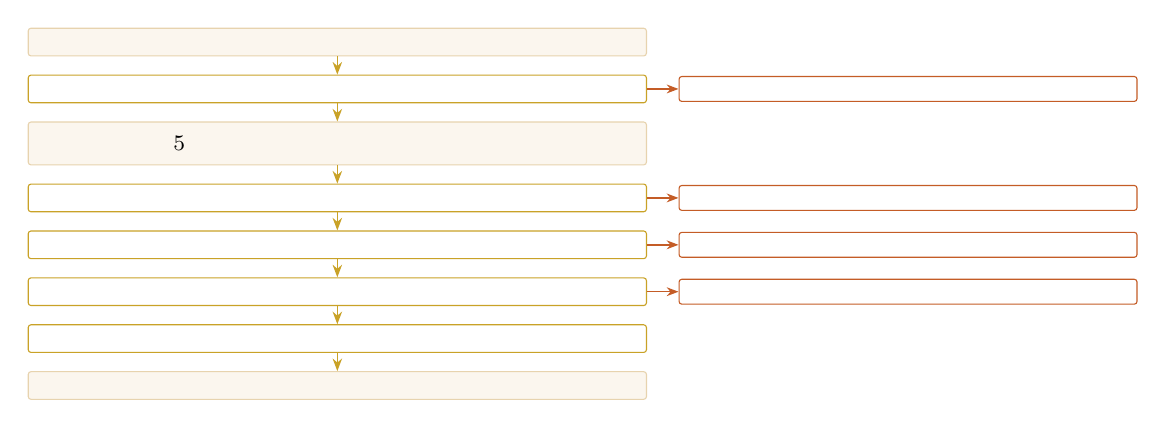
\begin{tikzpicture}[
  font=\footnotesize,
  zhstep/.style={draw=line, fill=cream, rounded corners=1pt, text width=7.5cm, align=left, inner sep=5pt},
  zhask/.style={draw=gold, fill=white, rounded corners=1pt, text width=7.5cm, align=left, inner sep=5pt},
  zhout/.style={draw=terra, fill=white, rounded corners=1pt, text width=5.5cm, align=left, inner sep=4.5pt},
  node distance=2.3mm and 4mm,
  arr/.style={gold, line width=0.6pt, -{Stealth[length=1.6mm]}}
]
  \node[zhstep] (a) {客户消息进入对话接口，先校验登录态};
  \node[zhask, below=of a] (b) {上一张确认卡仍待确认，且本句是肯定回复？};
  \node[zhout, right=of b] (b2) {重新展示该确认卡，请客户在卡片上输入交易密码};
  \node[zhstep, below=of b] (c) {按话题裁剪工具。主模型自主选择工具，最多 5 步；一旦生成卡片即停止};
  \node[zhask, below=of c] (d) {本句是要取回心愿备用金？};
  \node[zhout, right=of d] (d2) {按列表顺序生成取回确认卡；未指明第几笔则追问};
  \node[zhask, below=of d] (e) {主模型是否已经生成卡片？};
  \node[zhout, right=of e] (e2) {返回最后一张卡片};
  \node[zhask, below=of e] (f) {用途、金额、用钱日是否已由客户说全？};
  \node[zhout, right=of f] (f2) {生成心愿备用金确认卡};
  \node[zhask, below=of f] (g) {语义审核：漏调查看、虚假办结，或正常放行};
  \node[zhstep, below=of g] (h) {视审核结论补发查看卡片、改写尚未执行的话术，或在卡号与金额已齐时补转账确认卡};
  \draw[arr] (a) -- (b);
  \draw[arr] (b) -- (c);
  \draw[arr] (c) -- (d);
  \draw[arr] (d) -- (e);
  \draw[arr] (e) -- (f);
  \draw[arr] (f) -- (g);
  \draw[arr] (g) -- (h);
  \draw[terra, line width=0.5pt, -{Stealth[length=1.5mm]}] (b.east) -- (b2.west);
  \draw[terra, line width=0.5pt, -{Stealth[length=1.5mm]}] (d.east) -- (d2.west);
  \draw[terra, line width=0.5pt, -{Stealth[length=1.5mm]}] (e.east) -- (e2.west);
  \draw[terra, line width=0.5pt, -{Stealth[length=1.5mm]}] (f.east) -- (f2.west);
\end{tikzpicture}
\caption{对话处理流程}
\end{figure}

工具分为三类。

{\def\LTcaptype{none} % do not increment counter
\begin{longtable}[]{@{}
  >{\raggedright\arraybackslash}p{(\linewidth - 4\tabcolsep) * \real{0.3333}}
  >{\raggedright\arraybackslash}p{(\linewidth - 4\tabcolsep) * \real{0.3333}}
  >{\raggedright\arraybackslash}p{(\linewidth - 4\tabcolsep) * \real{0.3333}}@{}}
\toprule\noalign{}
\begin{minipage}[b]{\linewidth}\raggedright
类别
\end{minipage} & \begin{minipage}[b]{\linewidth}\raggedright
代表工具
\end{minipage} & \begin{minipage}[b]{\linewidth}\raggedright
对客户的效果
\end{minipage} \\
\midrule\noalign{}
\endhead
\specialrule{0.6pt}{0.45em}{0pt}
\endfoot
\bottomrule\noalign{}
\endlastfoot
只读取数 &
\texttt{get\_account\_overview}、\texttt{get\_spending\_breakdown}、\texttt{get\_risk\_and\_cashflow}、\texttt{get\_internal\_payees}
& 供模型组织文字说明，不直接作为固定视图 \\
固定视图 &
\texttt{show\_bill\_analysis}、\texttt{show\_bank\_cards}、\texttt{show\_wealth\_catalog}、\texttt{show\_security\_center}、\texttt{show\_wish\_reserves}
& 小程序渲染标准卡片 \\
办理预下单 &
\texttt{stage\_transfer}、\texttt{stage\_wealth\_purchase}、\texttt{stage\_card\_action}、\texttt{set\_up\_scenario}、\texttt{release\_scenario}、\texttt{cancel\_subscription}
& 生成待确认指令，此时不改余额 \\
\end{longtable}
}

客户谈论选购商品且语句中没有理财语义时，本轮从工具列表中移除理财货架、产品详情、配置建议和申购，避免日常消费被误办成理财。

\subsubsection{2.4
资金类业务的确认与入账}\label{ux8d44ux91d1ux7c7bux4e1aux52a1ux7684ux786eux8ba4ux4e0eux5165ux8d26}

对话阶段只产生状态为 \texttt{PENDING} 的指令，存放在进程内存。入账接口为
\texttt{POST\ /api/order/confirm}（与
\texttt{POST\ /api/transfer/confirm}
同一处理）。确认时再次校验登录态、指令归属、付款卡状态、限额和交易密码。校验通过后才调用账务函数。

\begin{figure}[htbp]
\centering
\begin{tikzpicture}[x=1cm,y=0.64cm]
  \node[font=\footnotesize\bfseries, text=golddeep] at (0,0.35) {客户};
  \node[font=\footnotesize\bfseries, text=golddeep] at (4.15,0.35) {小程序};
  \node[font=\footnotesize\bfseries, text=golddeep] at (8.3,0.35) {接入服务};
  \node[font=\footnotesize\bfseries, text=golddeep] at (12.45,0.35) {规则与账务};
  \draw[line, line width=0.6pt] (0,0.05) -- (0,-7.15);
  \draw[line, line width=0.6pt] (4.15,0.05) -- (4.15,-7.15);
  \draw[line, line width=0.6pt] (8.3,0.05) -- (8.3,-7.15);
  \draw[line, line width=0.6pt] (12.45,0.05) -- (12.45,-7.15);
  \draw[-{Stealth[length=1.5mm]}, terra] (0,-0.55) -- (4.15,-0.55);
  \node[font=\scriptsize, above] at (2.08,-0.55) {说明卡号与金额};
  \draw[-{Stealth[length=1.5mm]}, terra] (4.15,-1.35) -- (8.3,-1.35);
  \node[font=\scriptsize, above] at (6.22,-1.35) {提交对话};
  \draw[-{Stealth[length=1.5mm]}, terra] (8.3,-2.15) -- (12.45,-2.15);
  \node[font=\scriptsize, above] at (10.38,-2.15) {预校验限额与卡状态};
  \draw[-{Stealth[length=1.5mm]}, gold] (12.45,-2.95) -- (8.3,-2.95);
  \node[font=\scriptsize, above] at (10.38,-2.95) {可出卡，此时不扣款};
  \draw[-{Stealth[length=1.5mm]}, gold] (8.3,-3.75) -- (4.15,-3.75);
  \node[font=\scriptsize, above] at (6.22,-3.75) {展示确认卡};
  \draw[-{Stealth[length=1.5mm]}, terra] (0,-4.55) -- (4.15,-4.55);
  \node[font=\scriptsize, above] at (2.08,-4.55) {输入交易密码};
  \draw[-{Stealth[length=1.5mm]}, terra] (4.15,-5.35) -- (8.3,-5.35);
  \node[font=\scriptsize, above] at (6.22,-5.35) {提交确认};
  \draw[-{Stealth[length=1.5mm]}, terra] (8.3,-6.15) -- (12.45,-6.15);
  \node[font=\scriptsize, above] at (10.38,-6.15) {复核密码、限额与风险提示};
  \draw[-{Stealth[length=1.5mm]}, gold] (12.45,-6.95) -- (4.15,-6.95);
  \node[font=\scriptsize, above, fill=white, inner sep=1pt] at (8.3,-6.95) {入账后返回回执与最新余额};
\end{tikzpicture}
\caption{资金类业务的确认与入账。收款人为本行客户时，同一处理中贷记对方活期。}
\end{figure}

转账、理财申购、心愿备用金存入属于资金类指令，确认时必须校验交易密码。调整转账限额的指令同样要求交易密码。挂失、冻结、解冻按卡片操作规则执行。客户在对话中回复``确认''\,``好的''，只会使确认卡重新出现在对话底部，不能代替卡片上的密码确认。

\subsection{3. 核心算法说明}\label{ux6838ux5fc3ux7b97ux6cd5ux8bf4ux660e}

\subsubsection{3.1
对话编排与语义审核}\label{ux5bf9ux8bddux7f16ux6392ux4e0eux8bedux4e49ux5ba1ux6838}

主模型为 \texttt{Qwen/Qwen3.5-122B-A10B}，工具选择策略为自动，采样温度为
0.1，并关闭长思考，以保证工具调用的时延和稳定性。检查模型为
\texttt{Qwen/Qwen3.5-35B-A3B}。检查模型不可用时，回退到主模型。两路都无法返回合法结论时，保留主模型原文。

语义审核只在主模型本轮没有产出卡片、且给出了文字时启动。审核结论限于三种。

{\def\LTcaptype{none} % do not increment counter
\begin{longtable}[]{@{}
  >{\raggedright\arraybackslash}p{(\linewidth - 2\tabcolsep) * \real{0.5000}}
  >{\raggedright\arraybackslash}p{(\linewidth - 2\tabcolsep) * \real{0.5000}}@{}}
\toprule\noalign{}
\begin{minipage}[b]{\linewidth}\raggedright
结论
\end{minipage} & \begin{minipage}[b]{\linewidth}\raggedright
处理
\end{minipage} \\
\midrule\noalign{}
\endhead
\specialrule{0.6pt}{0.45em}{0pt}
\endfoot
\bottomrule\noalign{}
\endlastfoot
漏调查看工具 &
仅允许补调账单、银行卡、订阅、安全中心、理财画像、货架、产品详情、风险问卷、心愿备用金列表 \\
虚假办结 &
将``已经办理、已经冻结、已经生成确认单''等表述改写为尚未执行 \\
正常放行 & 保留追问、拒绝非银行业务或分析性说明 \\
\end{longtable}
}

审核模型不得代发转账、申购、存入或取回确认单，以免检查模型编造金额、日期或收款人。心愿备用金的用钱日以客户原话的日期解析结果为准。转账确认卡仅在客户原话中已经同时出现金额和储蓄卡卡号时补发。

会话历史按用户保存在进程内存，接口返回前保留最近 20
条。写入模型上下文时保留系统提示和最近 10
轮。卡片进入历史时只保留用途、金额、日期、产品名和``待客户点击确认''等摘要，便于后续指代。

\subsubsection{3.2
投资者风险承受能力评估}\label{ux6295ux8d44ux8005ux98ceux9669ux627fux53d7ux80fdux529bux8bc4ux4f30}

问卷共 11
题，覆盖年龄、家庭净资产、可投资产比例、当前配置、风险投资经验、投资态度、收益风险取舍、可接受期限、期望结果、波动焦虑和保本偏好。各选项分值在服务端维护，提交接口只接收选项字母，不接收客户端自报分值。

计分规则：

\[
S = \sum_{i=1}^{11} s(q_i)
\]

缺题时拒绝提交。总分按下列区间映射风险类型与产品等级。

{\def\LTcaptype{none} % do not increment counter
\begin{longtable}[]{@{}llll@{}}
\toprule\noalign{}
得分 & 风险类型 & 等级 & 可适配产品风险等级 \\
\midrule\noalign{}
\endhead
\specialrule{0.6pt}{0.45em}{0pt}
\endfoot
\bottomrule\noalign{}
\endlastfoot
15 分及以下 & 保守型 & R1 & 一级 \\
16--35 & 谨慎型 & R2 & 一级、二级 \\
36--60 & 稳健型 & R3 & 一级至三级 \\
61--80 & 进取型 & R4 & 一级至四级 \\
81--100 & 激进型 & R5 & 一级至五级 \\
\end{longtable}
}

年龄题同时写入年龄段，供银发识别和配置调整使用。职业由客户在问卷中选择，写入客户档案。测评日期为提交当日。自测评日起
365 日内视为有效。超过 365
日、等级为空或日期无法解析时，视为未持有有效测评。

适当性闸门作用于货架、单品详情、配置建议和申购预下单。产品风险等级数值高于客户等级时，详情与申购被拒绝，并向客户说明原因。系统在话术中声明理财非存款，不保证本金和收益。

\subsubsection{3.3 现金流画像}\label{ux73b0ux91d1ux6d41ux753bux50cf}

画像取近 90
日流水和当前活期余额。流水约定支出金额为正、收入金额为负。设观察期天数为
\(D\)，支出序列为 \(E\)，收入绝对值为 \(I\)，活期余额为 \(B\)。

\[
\text{月均支出} = \left(\sum E\right) \times \frac{30}{D}
\]

\[
\text{可投闲钱} = \max\left(B - 3 \times \text{月均支出},\, 0\right)
\]

\[
\text{周转率} = \frac{(\sum E + \sum I) / D}{\max(B,\, 1)}
\]

高周转：周转率不低于 0.04，或 90 日内流水不少于 12 笔。

闲钱沉淀：可投闲钱不低于 1,500 元，且支出标准差不超过支出均值的 0.8
倍。无支出样本时，只要求闲钱金额达标。

由此得到四种资金风格：高周转偏流动性、沉淀资金偏稳健锁期、活钱与锁期并存、均衡配置。银发客户按年龄段识别，年龄段包含
51--60、61--65、65 岁以上、60 岁以上或退休表述。

\subsubsection{3.4
资产配置比例}\label{ux8d44ux4ea7ux914dux7f6eux6bd4ux4f8b}

在客户风险等级对应的基准比例上做三项调整，再归一化到
100\%。每一档最低保留 5\%。前两档按比例四舍五入，第三档吸收舍入差额。

{\def\LTcaptype{none} % do not increment counter
\begin{longtable}[]{@{}llll@{}}
\toprule\noalign{}
等级 & 活钱管理 & 稳健增值 & 长期增值 \\
\midrule\noalign{}
\endhead
\specialrule{0.6pt}{0.45em}{0pt}
\endfoot
\bottomrule\noalign{}
\endlastfoot
R1 & 60\% & 35\% & 5\% \\
R2 & 50\% & 35\% & 15\% \\
R3 & 40\% & 35\% & 25\% \\
R4 & 30\% & 35\% & 35\% \\
R5 & 25\% & 30\% & 45\% \\
\end{longtable}
}

调整规则：

\begin{itemize}
\tightlist
\item
  高周转：活钱管理增加 10 个百分点，长期增值减少 10 个百分点。
\item
  闲钱沉淀：长期增值增加 10 个百分点，活钱管理减少 10 个百分点。
\item
  银发客户：活钱管理增加 15 个百分点，长期增值减少 15 个百分点。
\end{itemize}

未测评客户不套用默认等级，不给出配置比例。

\subsubsection{3.5
理财产品匹配}\label{ux7406ux8d22ux4ea7ux54c1ux5339ux914d}

候选集先按客户风险等级截断，只保留不高于客户等级的在售产品。若客户说明了这笔资金的使用时间，再按期限窗口过滤。窗口定义如下。

{\def\LTcaptype{none} % do not increment counter
\begin{longtable}[]{@{}ll@{}}
\toprule\noalign{}
客户表述 & 产品期限（天） \\
\midrule\noalign{}
\endhead
\specialrule{0.6pt}{0.45em}{0pt}
\endfoot
\bottomrule\noalign{}
\endlastfoot
活钱，随时可能使用 & 0 \\
七日，一周内用不上 & 0--7 \\
月度，一个月内用不上 & 7--30 \\
半年，半年内用不上 & 30--180 \\
年度，一年以上用不上 & 180--360 \\
\end{longtable}
}

过滤后若没有产品，则退回按风险等级截断后的全集，避免无结果。

单只产品基础分为
40。客户已经说明使用时间时，以该时间为主，不再用流水里的周转特征把客户推回短期产品。

\begin{itemize}
\tightlist
\item
  需要活钱：期限为 0 时加 30 分。
\item
  其他窗口：设窗口上沿为 \(H\)、产品期限为 \(T\)，加分为
  \(\max(0,\, 24 - \lfloor |H-T| / 7 \rfloor)\)。
\item
  未说明使用时间时：高周转或自由职业类职业优先 7 日内产品（加 35 分）和
  30 日内产品（加 8 分）；闲钱沉淀优先 30--90 日（加 32 分）和 180
  日以上（加 10 分）；收支平稳时 30 日内产品加 15 分。
\item
  银发客户：期限不超过 90 日且产品风险不高于 R2 时加 12 分；期限达到 360
  日扣 8 分。
\item
  产品风险与客户等级相同加 4 分；活期类产品加 2 分。
\item
  已持有同一产品扣 12 分，并在理由中说明可加仓或换期限搭配。
\end{itemize}

排序键为匹配分降序、期限升序、参考收益降序，保证相同输入下结果稳定。随后做期限分散：先按持有期分档各取一只最高分产品，分档为活期、超短、短期、中期、长期，再用剩余高分产品补足默认
3 只。

推荐说明按``测评依据、闲钱测算、期限搭配、已持仓回避''组织，并请客户确认是否调整。闲钱为
0 时，说明按约 3 个月支出预留备用金，建议从活钱类产品起步。

\subsubsection{3.6
转账风险识别}\label{ux8f6cux8d26ux98ceux9669ux8bc6ux522b}

风险识别在生成确认卡和密码确认两个时点执行。确认时若等级不是正常，客户须在界面确认已阅读提示，否则拒绝入账。识别使用最近
12 笔转出和近 24 小时转入。大额阈值为单笔 2,000 元。

{\def\LTcaptype{none} % do not increment counter
\begin{longtable}[]{@{}
  >{\raggedright\arraybackslash}p{(\linewidth - 4\tabcolsep) * \real{0.3333}}
  >{\raggedright\arraybackslash}p{(\linewidth - 4\tabcolsep) * \real{0.3333}}
  >{\raggedright\arraybackslash}p{(\linewidth - 4\tabcolsep) * \real{0.3333}}@{}}
\toprule\noalign{}
\begin{minipage}[b]{\linewidth}\raggedright
信号
\end{minipage} & \begin{minipage}[b]{\linewidth}\raggedright
触发条件
\end{minipage} & \begin{minipage}[b]{\linewidth}\raggedright
等级
\end{minipage} \\
\midrule\noalign{}
\endhead
\specialrule{0.6pt}{0.45em}{0pt}
\endfoot
\bottomrule\noalign{}
\endlastfoot
连续大额 & 本笔不低于 2,000 元，且近 72 小时已有同样量级的转出 & 高 \\
单笔大额 & 本笔不低于 5,000 元，且未构成连续大额 & 关注 \\
首次大额收款人 & 本笔不低于 2,000 元，且收款人未出现在近期转出对手中 &
至少为关注 \\
当日高频 & 本笔不低于 2,000 元，且当日已有不少于 5 笔转出 &
至少为关注 \\
夜间大额 & 本笔不低于 2,000 元，且当地时间处于 0 时至 6 时 &
至少为关注 \\
整数大额 & 本笔不低于 10,000 元，且金额为 1,000 元的整数倍 &
至少为关注 \\
快进快出 & 本笔不低于 2,000 元，且近 24 小时存在转入 & 至少为关注 \\
\end{longtable}
}

多个信号可以叠加。连续大额优先生成为高等级，其余信号在尚未定级时定为关注。等级为高时，若客户已绑定紧急联系人，入账成功后写入一条预警记录，并在回执中告知已通知联系人。当前实现将预警记入本系统，不发送真实短信或微信模板消息。

\subsubsection{3.7 转账限额}\label{ux8f6cux8d26ux9650ux989d}

付款工具必须是状态正常的储蓄卡。信用卡、冻结卡、挂失卡和状态异常卡不能付款。收款侧拒绝信用卡和本人账户。卡号格式正确但不是本行账户时，演示环境只扣减付款人余额并登记流水，不向行外清算。

限额按付款卡统计当日金额、当日笔数和当年金额。默认储蓄卡限额为：单笔
20,000 元、日累计 20,000 元、日累计 10 笔、年累计 2,000,000
元。种子客户可按客群设置不同额度。客户自助调额不得超过单笔 500,000
元、日累计 1,000,000 元、日累计 100 笔、年累计 50,000,000 元。

校验顺序为：卡片存在且为正常储蓄卡、金额大于
0、单笔、日笔数、日金额、年金额、活期余额。任一项不满足即拒绝，并给出可执行的调额引导。本笔之后剩余日累计或年累计低于上限的
20\%，或日笔数已经用尽时，交易仍可成功，同时在确认信息中给出临界提示。

确认接口在扣款前重新执行上述校验，防止仅依赖前端展示。

\subsubsection{3.8
心愿备用金日程与参考收益}\label{ux5fc3ux613fux5907ux7528ux91d1ux65e5ux7a0bux4e0eux53c2ux8003ux6536ux76ca}

心愿备用金把一笔活期资金单独登记到指定用钱日。客户必须自己说出用途、金额和今天之后的用钱日。受益人可选，客户未说明时不追问。日期解析支持公历日期、本月或下月某日、明天至大后天，以及本周、下周、下下周的星期。模型补写的日期不作为用钱日。

赎回日算法：

\begin{enumerate}
\def\labelenumi{\arabic{enumi}.}
\tightlist
\item
  用钱日若落在周末或法定假日，先对齐到前一个工作日，记为资金须就绪日。
\item
  自就绪日向前数 3
  个工作日，得到计划赎回日。工作日为周一至周五，并扣除内置的国务院放假日期。调休上班的周末仍按非工作日处理，使赎回只可能提前。
\item
  若计划赎回日不晚于今天，则把赎回日改为就绪日与下一工作日中的较晚者，避免客户刚确认就被调度线程赎回。
\item
  若调整后的赎回日仍晚于就绪日，说明用钱日过近、资金赶不上使用，拒绝建单。
\end{enumerate}

计息起点：当地时间 15:00 以前确认为当日；当日不是工作日，或确认时点在
15:00 及以后，则顺延到下一工作日。底层产品固定为在售的 R1
现金管理产品。参考收益按交易日计提：

\[
\Delta = P \times \frac{y}{365} \times n
\]

其中 \(P\) 为当前本金，\(y\) 为产品参考年化，\(n\)
为自上一个计息点至本交易日的自然日数。周末和法定假日并入下一交易日，不单独计息。收益记入专款台账，赎回或提前取回时与本金一并回到可用余额。系统向客户说明该收益为参考计提，不构成保本或收益承诺。

调度线程约每 30
秒按服务器当地日期检查。赎回日当天将本息划回可用余额，状态改为已完成，并写入未读提醒。用钱日当天若已经完成赎回，再提醒一次可以按计划使用。小程序在页面打开时轮询未读提醒。提前取回须经确认卡和交易密码，成功后状态改为提前结束，本息立即回到可用余额，后续不再做用钱日提醒。

存续列表按用钱日、同一天再按创建时间排序。客户说``第几笔''时按该顺序定位，第一笔序号为
1。

\subsubsection{3.9
账单时间窗口}\label{ux8d26ux5355ux65f6ux95f4ux7a97ux53e3}

客户未说明时间时，支出分析取近 30
日。客户只说月份、未说年份时，由服务端按当天判断：该月已经到来则使用今年，尚未到来则使用去年。客户明确说出今年、去年或具体年份时，才把年份传入工具。异常交易由服务端根据金额偏离识别，供账单卡片展示。

\subsection{4. 安全设计}\label{ux5b89ux5168ux8bbeux8ba1}

\subsubsection{4.1 安全目标}\label{ux5b89ux5168ux76eeux6807}

{\def\LTcaptype{none} % do not increment counter
\begin{longtable}[]{@{}
  >{\raggedright\arraybackslash}p{(\linewidth - 2\tabcolsep) * \real{0.5000}}
  >{\raggedright\arraybackslash}p{(\linewidth - 2\tabcolsep) * \real{0.5000}}@{}}
\toprule\noalign{}
\begin{minipage}[b]{\linewidth}\raggedright
目标
\end{minipage} & \begin{minipage}[b]{\linewidth}\raggedright
系统中的落实方式
\end{minipage} \\
\midrule\noalign{}
\endhead
\specialrule{0.6pt}{0.45em}{0pt}
\endfoot
\bottomrule\noalign{}
\endlastfoot
身份可信 & 账号口令校验后签发会话凭证，业务接口校验凭证与客户号一致 \\
资金操作可确认 & 资金类指令二次校验交易密码、付款卡和限额 \\
职责分离 & 模型不能直接改写余额、限额、风险等级和订单状态 \\
适当性 & 测评有效期和产品风险等级由服务端比较 \\
欺诈提示 &
规则识别大额、夜间、高频、快进快出等特征，高风险留痕并通知紧急联系人 \\
最小展示 & 登录响应返回脱敏手机号；对话不索取交易密码 \\
可解释 & 拒绝原因、剩余额度和风险提示返回给渠道，供客户阅读 \\
\end{longtable}
}

\subsubsection{4.2
身份鉴别与会话}\label{ux8eabux4efdux9274ux522bux4e0eux4f1aux8bdd}

客户使用手机号或客户号加登录密码进入系统。口令不以明文存放。存储值为固定盐与口令拼接后的
SHA-256 摘要。登录成功后签发 128
位随机凭证，保存在进程内存，后续请求必须同时提交客户号和凭证。凭证与客户号不一致时返回未授权。退出登录时删除凭证。

交易密码与登录密码使用同一套摘要校验。演示数据中两者均为同一初始口令。资金类确认和限额调整在服务端重新校验，不信任渠道自行声明的``已验证''。

手机号对外展示时保留前三后四。紧急联系人手机号按同一规则脱敏。

\subsubsection{4.3 交易完整性}\label{ux4ea4ux6613ux5b8cux6574ux6027}

待确认指令包含客户号、业务类型、金额、对手或产品、付款卡和状态。确认时核对指令仍为待确认，且属于当前客户。客户可以撤销尚未确认的指令。

入账函数在数据库事务中更新余额和流水。心愿备用金同时减少可用余额、增加锁定资金，并写入专款主记录和申购明细。可用余额不足时整笔失败，不产生部分扣款。本行储蓄卡之间转账在同一处理中贷记收款人活期。

模型上下文不包含交易密码。系统提示明确要求模型不得在对话中索要密码。语义审核的改写结果同样禁止出现索要密码的语句。

\subsubsection{4.4
模型使用边界}\label{ux6a21ux578bux4f7fux7528ux8fb9ux754c}

发送给推理服务的内容包括系统提示、近期对话摘要和工具返回的业务数据。工具返回用于让模型组织下一句说明。下列事项不交给模型决定：

\begin{itemize}
\tightlist
\item
  是否扣减余额或锁定资金；
\item
  限额是否足够、卡片是否可付；
\item
  风险测评分数和等级；
\item
  产品是否超出客户风险等级；
\item
  心愿备用金的赎回日和计息结果；
\item
  交易密码是否正确。
\end{itemize}

工具说明中不放置具体客户姓名、卡号或手机号示例，避免模型把示例数据写入当前客户的备注或对手信息。用途、受益人、收款卡号和商户名要求照录客户原话。

\subsubsection{4.5 数据与密钥}\label{ux6570ux636eux4e0eux5bc6ux94a5}

业务数据存放在服务端本地 SQLite 数据库，路径固定为后端目录下的
\texttt{bank.db}，避免因启动目录不同生成多份账本。模型访问密钥从环境变量读取。密钥、数据库文件和语音缓存不应纳入版本库。

适老版语音优先调用外部神经网络语音，并按文本与音色缓存结果。外部连接失败时，本次改用操作系统语音合成，下一句仍优先尝试神经网络语音。

\subsubsection{4.6
隐私与适老保护}\label{ux9690ux79c1ux4e0eux9002ux8001ux4fddux62a4}

银发客户登录后，渠道默认使用适老界面。安全中心展示紧急联系人绑定状态、历史预警和防骗提示。绑定联系人必须提供姓名和合法手机号，关系限于子女、父母、配偶、亲属或其他。

高风险转账的通知对象是客户本人绑定的联系人。通知内容包含风险标题、收款人和金额。演示环境只在本系统留存记录并在回执中展示，不向运营商或即时通讯渠道外发。

\subsubsection{4.7
演示环境与投产要求}\label{ux6f14ux793aux73afux5883ux4e0eux6295ux4ea7ux8981ux6c42}

下列事项是当前演示实现的客观边界。若进入银行生产或准生产，应在现有业务闭环之上替换为行内标准控制，而不改变``模型不直接入账''的架构。

{\def\LTcaptype{none} % do not increment counter
\begin{longtable}[]{@{}
  >{\raggedright\arraybackslash}p{(\linewidth - 4\tabcolsep) * \real{0.3333}}
  >{\raggedright\arraybackslash}p{(\linewidth - 4\tabcolsep) * \real{0.3333}}
  >{\raggedright\arraybackslash}p{(\linewidth - 4\tabcolsep) * \real{0.3333}}@{}}
\toprule\noalign{}
\begin{minipage}[b]{\linewidth}\raggedright
领域
\end{minipage} & \begin{minipage}[b]{\linewidth}\raggedright
当前演示实现
\end{minipage} & \begin{minipage}[b]{\linewidth}\raggedright
投产时应达到的控制
\end{minipage} \\
\midrule\noalign{}
\endhead
\specialrule{0.6pt}{0.45em}{0pt}
\endfoot
\bottomrule\noalign{}
\endlastfoot
口令存储 & 固定盐 SHA-256，登录口令与交易口令同一摘要 &
分项口令、慢哈希或硬件加密，并实施错误次数锁定 \\
会话 & 进程内存凭证，服务重启即失效，无独立有效期和设备绑定 &
集中会话、空闲超时、绝对超时、退出全端失效 \\
传输 & 本地明文 HTTP & 全链路 TLS，渠道证书校验 \\
指令与会话 & 待确认指令和对话历史在进程内存 &
持久化、幂等、超时作废，并纳入交易审计 \\
账务 & 单机 SQLite & 行内核心或账务中台，借贷平衡与日终对账 \\
行外转账 & 仅扣减演示账户 & 接入支付清算与收款行校验 \\
模型数据 & 对话与工具结果发往外部推理服务 &
行内模型或专有云，数据出境与脱敏评估，提示词与输出审计 \\
密钥 & 环境变量中的推理密钥 & 密钥管理系统、定期轮换、最小权限 \\
紧急联系人通知 & 系统内记录 & 经行内消息平台发送，并记录送达回执 \\
反欺诈 & 固定阈值规则 & 与行内反欺诈、反洗钱名单和设备指纹联动 \\
语音 & 外部语音服务，失败回退本机 & 行内语音能力，文本脱敏后送入 \\
高可用与审计 & 单进程 & 多实例、操作日志、模型调用日志和管理员审计 \\
\end{longtable}
}

\subsubsection{4.8
已知风险的处理立场}\label{ux5df2ux77e5ux98ceux9669ux7684ux5904ux7406ux7acbux573a}

演示数据库中的初始口令仅用于功能演示，不得作为任何真实客户的口令策略。推理密钥若出现在本地配置文件中，只允许留在运行机器，不得提交到代码仓库或写入本说明书。外部推理服务能够看到客户对话中的账户摘要、金额和对手信息，因此本系统在完成数据出境评估前，只应用于脱敏演示数据。

\subsection{5. 主要接口}\label{ux4e3bux8981ux63a5ux53e3}

除特别说明外，业务接口均要求有效登录凭证，且凭证绑定的客户号与请求客户号一致。

{\def\LTcaptype{none} % do not increment counter
\begin{longtable}[]{@{}
  >{\raggedright\arraybackslash}p{(\linewidth - 4\tabcolsep) * \real{0.3333}}
  >{\raggedright\arraybackslash}p{(\linewidth - 4\tabcolsep) * \real{0.3333}}
  >{\raggedright\arraybackslash}p{(\linewidth - 4\tabcolsep) * \real{0.3333}}@{}}
\toprule\noalign{}
\begin{minipage}[b]{\linewidth}\raggedright
方法
\end{minipage} & \begin{minipage}[b]{\linewidth}\raggedright
路径
\end{minipage} & \begin{minipage}[b]{\linewidth}\raggedright
作用
\end{minipage} \\
\midrule\noalign{}
\endhead
\specialrule{0.6pt}{0.45em}{0pt}
\endfoot
\bottomrule\noalign{}
\endlastfoot
POST & \texttt{/api/auth/login} &
校验账号口令，返回凭证、脱敏资料、风险等级、是否银发、紧急联系人状态和余额 \\
POST & \texttt{/api/auth/logout} & 注销凭证 \\
POST & \texttt{/api/chat} & 提交一句话，返回文字或卡片，并附当前余额 \\
POST & \texttt{/api/order/confirm} & 校验密码后执行待确认指令 \\
POST & \texttt{/api/order/cancel} & 撤销待确认指令 \\
POST & \texttt{/api/risk/survey} &
提交问卷选项，服务端计分并返回配置建议 \\
GET & \texttt{/api/user/balance} & 查询活期余额 \\
GET & \texttt{/api/scenario/notices} & 拉取未读的到账提醒和用钱日提醒 \\
POST & \texttt{/api/scenario/notices/read} & 将提醒标记为已读 \\
GET & \texttt{/api/guardian/center} & 查询安全防护信息 \\
POST & \texttt{/api/guardian/bind} & 绑定或更新紧急联系人 \\
GET & \texttt{/api/tts} & 将指定文本合成为语音 \\
\end{longtable}
}

\subsection{6. 主要数据}\label{ux4e3bux8981ux6570ux636e}

{\def\LTcaptype{none} % do not increment counter
\begin{longtable}[]{@{}
  >{\raggedright\arraybackslash}p{(\linewidth - 2\tabcolsep) * \real{0.5000}}
  >{\raggedright\arraybackslash}p{(\linewidth - 2\tabcolsep) * \real{0.5000}}@{}}
\toprule\noalign{}
\begin{minipage}[b]{\linewidth}\raggedright
数据
\end{minipage} & \begin{minipage}[b]{\linewidth}\raggedright
内容
\end{minipage} \\
\midrule\noalign{}
\endhead
\specialrule{0.6pt}{0.45em}{0pt}
\endfoot
\bottomrule\noalign{}
\endlastfoot
客户 &
客户号、姓名、手机号、口令摘要、风险等级、风险类型、得分、测评日期、年龄段、职业、问卷原文、紧急联系人 \\
账户 & 可用余额、锁定资金 \\
银行卡 & 卡种、状态、单笔限额、日累计金额、日累计笔数、年累计金额 \\
流水 & 金额、分类、对手、附言、时间、付款卡 \\
理财产品 & 风险等级、期限、参考收益、起购金额、销售状态 \\
订阅 & 商户、金额、周期、下次扣款日、状态 \\
心愿备用金 & 用途、本金、累计参考收益、用钱日、赎回日、计息日、状态 \\
专款明细 & 申购、收益计提、赎回或提前结束 \\
提醒与预警 & 未读提醒、紧急联系人预警记录 \\
\end{longtable}
}

心愿备用金状态包括存续、已完成和提前结束。列表对已完成和提前结束作出标注，避免被理解为正常持有到期。

\subsection{7. 汇报结论}\label{ux6c47ux62a5ux7ed3ux8bba}

本系统已经形成可演示的零售对话闭环：渠道采集客户语言，模型选择业务工具，服务端规则决定是否出卡和是否入账，客户在确认卡上完成资金授权。风险测评、产品适当性、转账限额、反欺诈提示、紧急联系人留痕和心愿备用金日程均由确定性程序执行，模型不能绕过这些控制直接改账。

作为向银行专业部门的汇报材料，应同时明确其边界。当前实现用于验证业务与架构，口令学、会话、传输、账务一致性、模型数据驻留和外部通知仍停留在演示强度。生产化的工作重点是把上述控制替换为行内标准组件，并保留``自然语言受理、规则裁决、客户确认后入账''这一职责划分。

\end{document}
